%  Template for ICASSP-2021 paper; to be used with:
%          spconf.sty  - ICASSP/ICIP LaTeX style file, and
%          IEEEbib.bst - IEEE bibliography style file.
% --------------------------------------------------------------------------
\documentclass{article}
\usepackage{spconf,amsmath,graphicx}

% Example definitions.
% --------------------
\def\x{{\mathbf x}}
\def\L{{\cal L}}

% Title.
% ------
\title{AIML 425 Assignemnt 1}
%
% Single address.
% ---------------
\name{Quan Zhao (Student ID: 300471028)}
%\name{Author(s) Name(s)\thanks{Thanks to XYZ agency for funding.}}
\address{Victoria University of Wellington}
%
% For example:
% ------------
%\address{School\\
%	Department\\
%	Address}
%
% Two addresses (uncomment and modify for two-address case).
% ----------------------------------------------------------
%\twoauthors
%  {A. Author-one, B. Author-two\sthanks{Thanks to XYZ agency for funding.}}
%	{School A-B\\
%	Department A-B\\
%	Address A-B}
%  {C. Author-three, D. Author-four\sthanks{The fourth author performed the work
%	while at ...}}
%	{School C-D\\
%	Department C-D\\
%	Address C-D}
%
\begin{document}
%\ninept
%
\maketitle
%
\section{Introduction}
\label{sec:intro}

Generative models are a subset of machine learning models designed to capture and mimic the underlying distribution of the data on which they are trained. They can produce new samples that resemble the input data but might not have been part of the original training set.

In this work, I will present my understanding of training and tuning generative models.

Three models will be trained:

1. The first model, $f1$, has an input that follows a 2D Gaussian distribution and produces an output following a 2D uniform distribution.

2. The second model, $f2$, takes the output of model $f1$ as its input and produces an output that follows a 2D Gaussian distribution.

3. The third model, $f3$, accepts an input that follows a 1D uniform distribution and generates an output following a 2D Gaussian distribution.

We have introduced experiments to discuss:

  - The effects of varying levels of L2 regularization on the weights for $f1$.
  
  - The implications of concatenating the two networks, $f1$ and $f2$.

Finally, we will showcase the point mapping from the input to the output of model $f3$.

% Below is an example of how to insert images. Delete the ``\vspace'' line,
% uncomment the preceding line ``\centerline...'' and replace ``imageX.ps''
% with a suitable PostScript file name.
% -------------------------------------------------------------------------
\begin{figure}[htb]
  %
  \begin{minipage}[a]{.48\linewidth}
    \centering
    \centerline{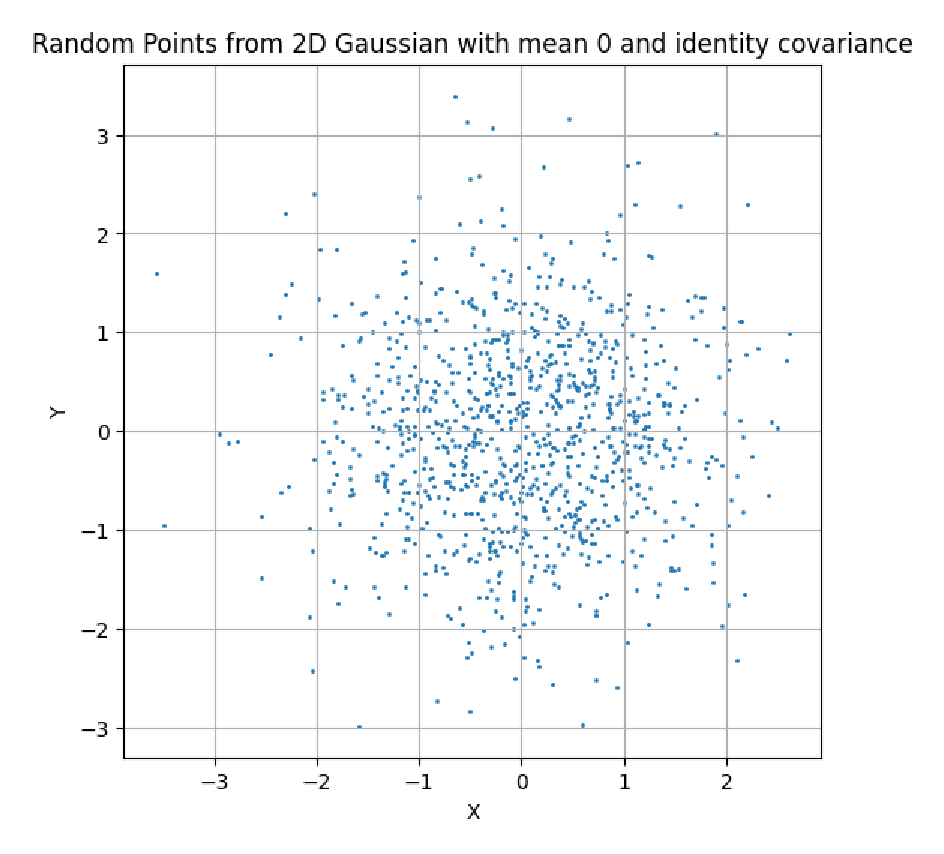
\includegraphics[width=3.0cm]{images/gaussian2d}}
  %  \vspace{1.5cm}
    \centerline{(a) 2D Gaussian distribution}\medskip
  \end{minipage}
  \hfill
  \begin{minipage}[c]{0.48\linewidth}
    \centering
    \centerline{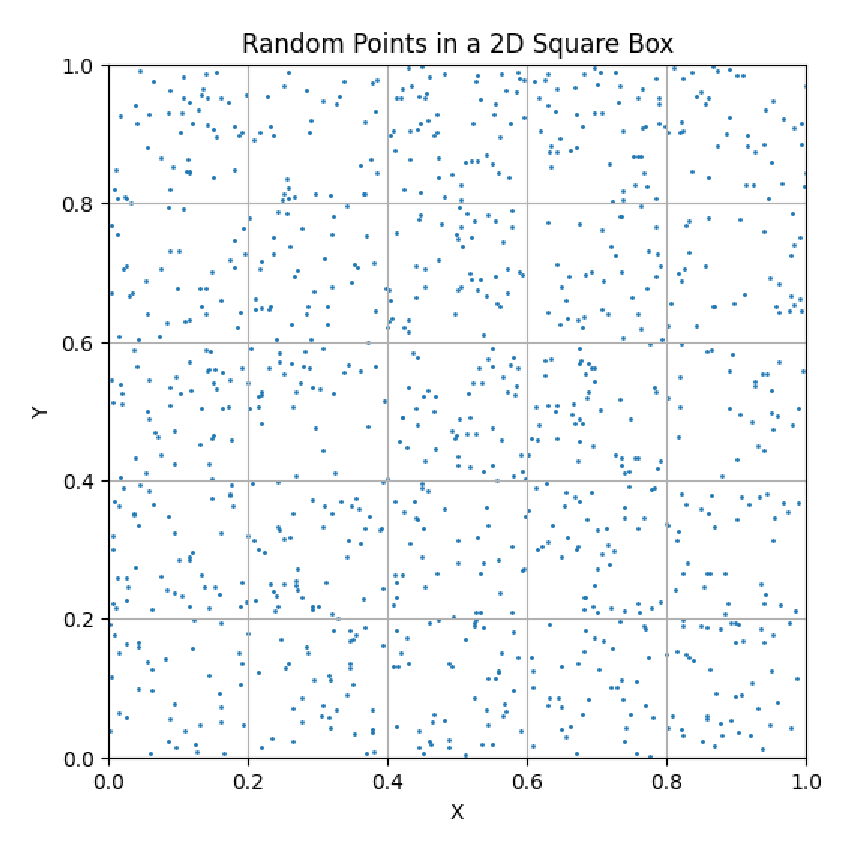
\includegraphics[width=2.7cm]{images/uniform2d}}
  %  \vspace{1.5cm}
    \centerline{(b) 2D uniform distribution}\medskip
  \end{minipage}
  %
  \caption{Data distribution plots}
  \label{fig:res}
  %
  \end{figure}
  

\section{THEORY}
\label{sec:theory}

\subsection{MMD}
\label{ssec:mmd}

Maximum Mean Discrepancy (MMD) is a statistical test for determining whether two samples come from the same distribution. It's often used in the context of kernel methods and has applications in training generative models.

$ \text{MMD}^2 = E[k(x, x')] + E[k(y, y')] - 2E[k(x, y)] $

where, $k(.,.)$ is the kernel function. 
$x, x'$ are independent samples from $X$,
and $y, y'$ are independent samples from $Y$.

\subsubsection{Kernel}
\label{sssec:kernel}

A common choice of kernel for MMD is the Gaussian (RBF) kernel:

$ k(x, y) = \exp\left(-\frac{||x - y||^2}{r}\right) $

Where, $r$ is chosen by designer



\subsection{L2 Regularization}
\label{ssec:l2regularization}

L2 regularization introduces a penalty on the squared magnitudes of model weights. 
In Nerual Networks, the loss function with L2 regularization is:

$ J(\theta) = \text{MMD}(\theta) + \lambda ||\theta||_2^2 $

Where,

- $\lambda$ is the regularization strength

- $||\theta||_2^2$ is the L2 norm of the parameter vector.

\section{RESULTS}
\label{sec:results}

\subsection{Train a fully connected neural network $f1$ of your design that converts a
two-dimensional (2D) $Z \sim N (0, I)$ into a 2D uniform $Y$ . That is, $Y$ has
a uniform density of 1 in a 2D square box (2-cube; edges have length 1).}
\label{ssec:q1}

A 3 fully-connected layers nerual network is been used train this model, 
which use MMD is Loss function with Gaussian Kernel. 
Gradient Descent Learning algorithms use Adam.

From Figure $\ref{fig:f1}$ we can see the input points are good mapping to the predicate points.

\begin{figure}[htb]

  \begin{minipage}[b]{1.0\linewidth}
    \centering
    \centerline{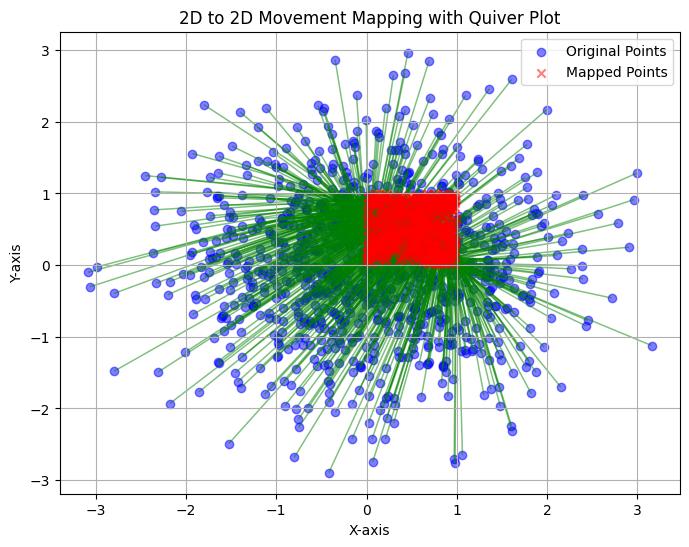
\includegraphics[width=6.5cm]{images/f1}}
  %  \vspace{2.0cm}
    \centerline{(a) Result 1}\medskip
  \end{minipage}
  %
  \caption{Points movement from input to predicate points}
  \label{fig:f1}
  %
  \end{figure}

\subsection{Train a second network $f2$ that converts the 2D $Y$ into a Gaussian 2D $Z$}
\label{ssec:q2}

pass

\subsection{Train $f1$ with different levels of $L2$ regularization on the weights and
discuss the effect.}
\label{ssec:q3}

We conducted experiments using the $f1$ model by adjusting the $L2$ regularization values. 
The specific values tested were: 

$
1\times 10^{-1}, 1\times 10^{-2}, 
1\times 10^{-3}, 1\times 10^{-4}, 1\times 10^{-5}, 
1\times 10^{-6}, 1\times 10^{-7}, 1\times 10^{-8}, 
1\times 10^{-10}, 1\times 10^{-15}, 1\times 10^{-20} 
$ 

Figure $\ref{fig:q3}$ a highlights the behavior of 
the average loss across these regularization values. 
There's a pronounced reduction in loss after 
$1\times 10^{-2}$. However, post 
$1\times 10^{-4}$, the loss remains relatively stable without significant fluctuations.

The evolution in point mapping becomes evident when examining 
Figures $\ref{fig:q3}$ b through $\ref{fig:q3}$  e, it shows point mapping to one point,
after weight increased it teand to mapping to a line.

after $1\times 10^{-4}$, input points have good mapping shape is stable and same to output shape.


\begin{figure}[htb]

  \begin{minipage}[b]{1.0\linewidth}
    \centering
    \centerline{\includegraphics[width=8.0cm]{images/q3_1}}
   %\vspace{2.0cm}
   \centerline{(a) $f1$ Avg Loss with diff L2 weight decay }\medskip
  \end{minipage}
  %
  \begin{minipage}[b]{.48\linewidth}
    \centering
    \centerline{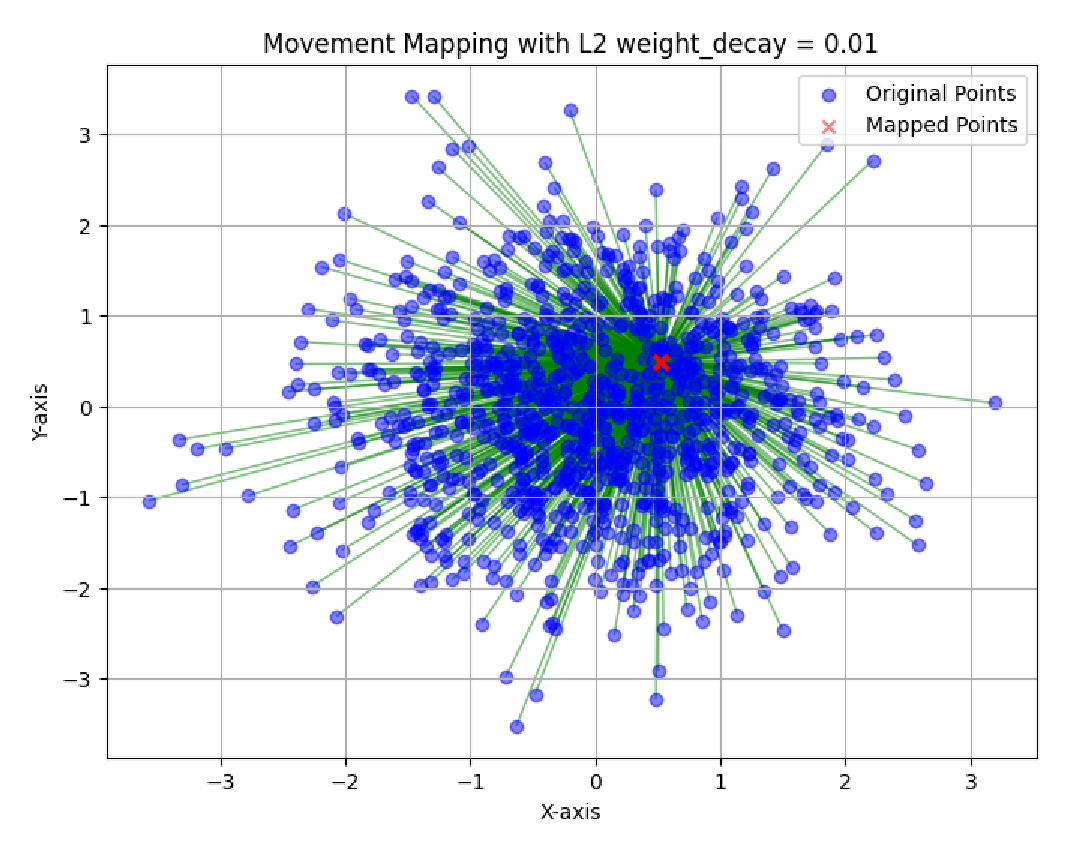
\includegraphics[width=3.0cm]{images/q3_1e-2}}
  %  \vspace{1.5cm}
    \centerline{(b) Points movement with 1e-2}\medskip
  \end{minipage}
  \hfill
  \begin{minipage}[b]{0.48\linewidth}
    \centering
    \centerline{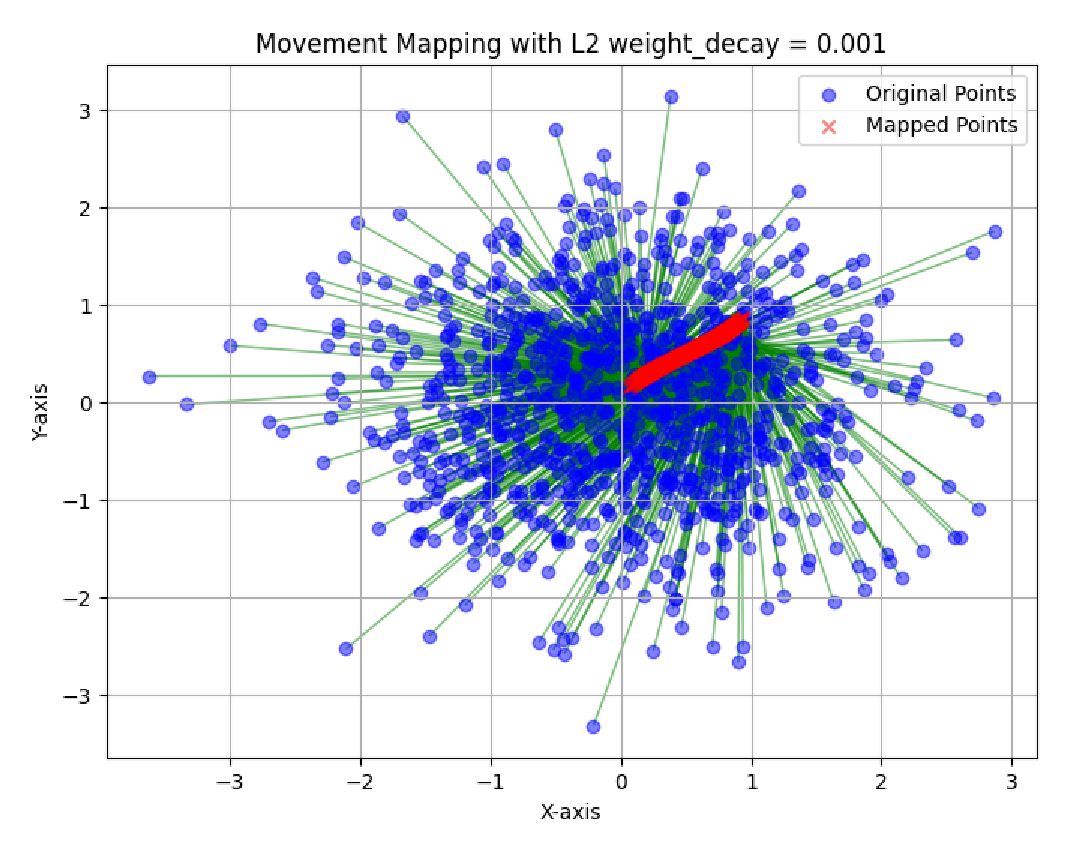
\includegraphics[width=3.0cm]{images/q3_1e-3}}
  %  \vspace{1.5cm}
    \centerline{(c) Points movement with 1e-3}\medskip
  \end{minipage}
  %
  %
  \begin{minipage}[b]{.48\linewidth}
    \centering
    \centerline{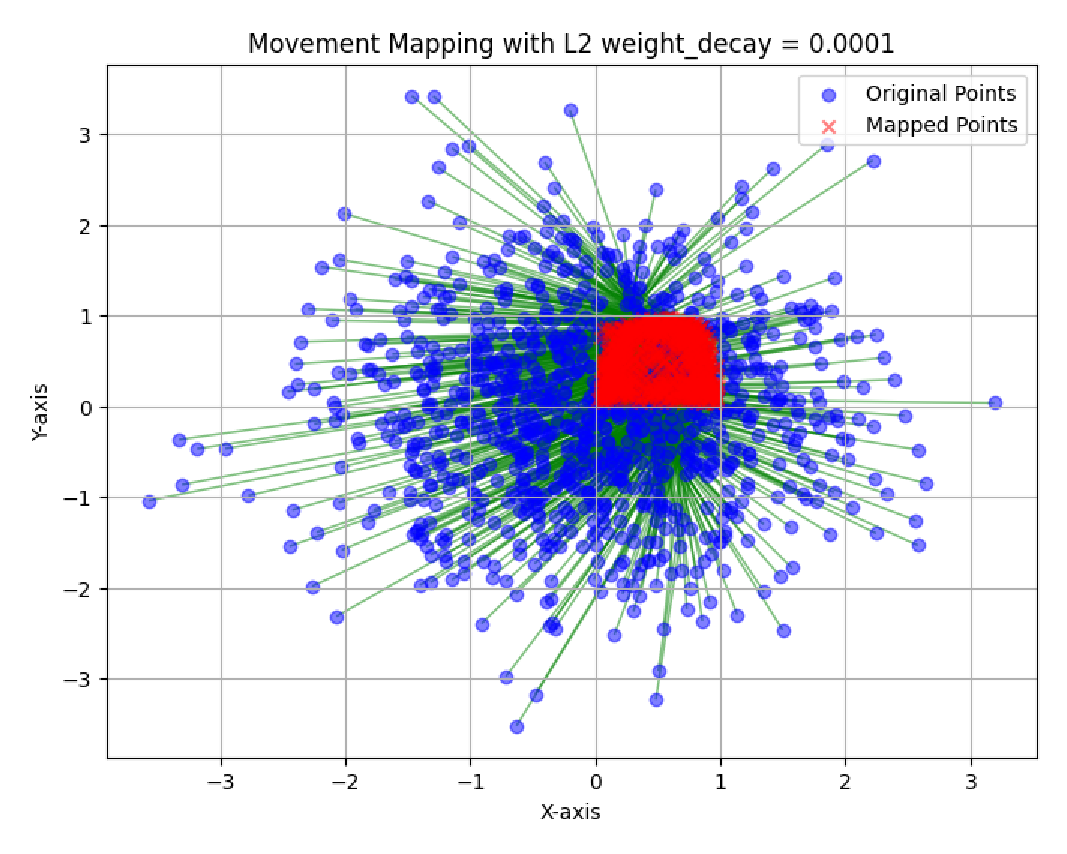
\includegraphics[width=3.0cm]{images/q3_1e-4}}
  %  \vspace{1.5cm}
    \centerline{(d) Points movement with 1e-4}\medskip
  \end{minipage}
  \hfill
  \begin{minipage}[b]{0.48\linewidth}
    \centering
    \centerline{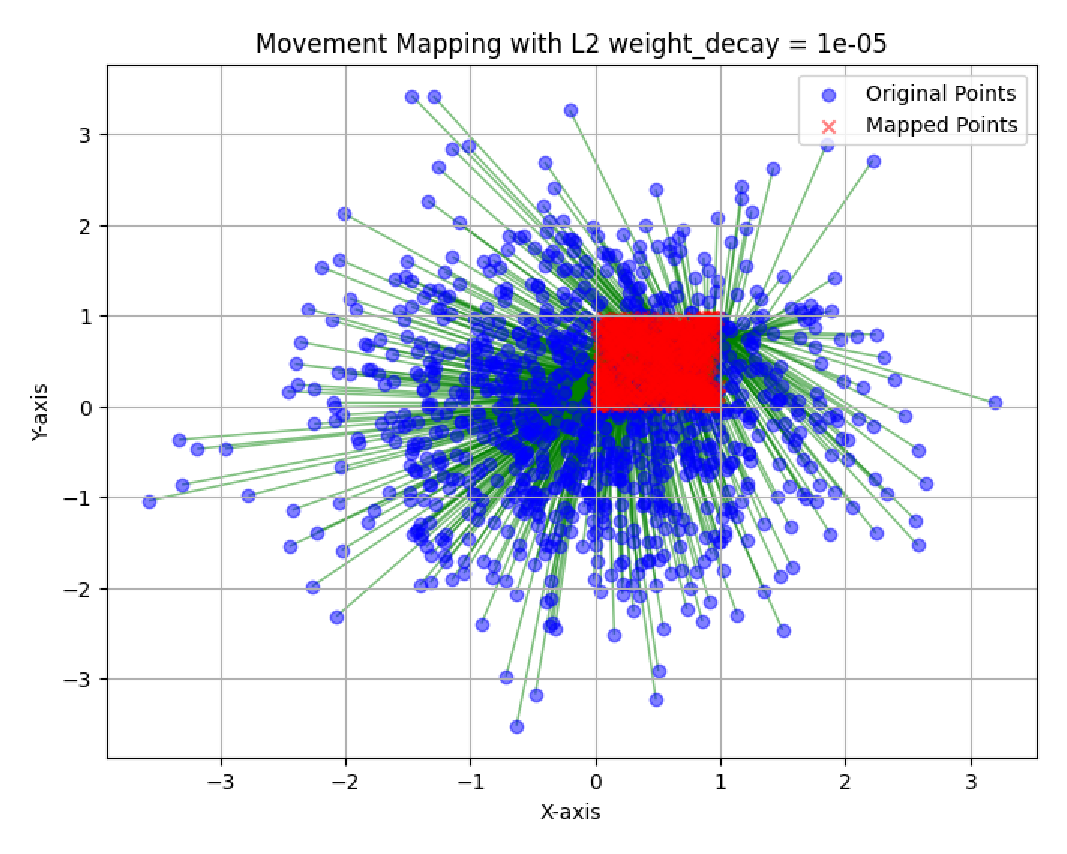
\includegraphics[width=3.0cm]{images/q3_1e-5}}
  %  \vspace{1.5cm}
    \centerline{(e) Points movement with 1e-5}\medskip
  \end{minipage}
  %
  \caption{visulization of dataset}
  \label{fig:q3}
  %
  \end{figure}

\subsection{Using colour plots (various options), discuss what happens to individual
input data points if we concatenate two networks $f2$ ◦ $f1$ (mapping
Gaussian to Gaussian) with different $L2$ regularizations. Discuss the
movement of adjacent points and the effect of the regularization.}
\label{ssec:q4}

pass

\subsection{Train a third network $f3$ that converts a 1D uniform $Y$ into a gaussian
2D $Z$. Again use colour plots that show how points are mapped from
the input $Y$ to the output $Z$}
\label{ssec:q5}

We've trained the model $f3$, using a neural network that consists of three fully-connected layers. To evaluate the model's performance, we employed the Maximum Mean Discrepancy (MMD) with a Gaussian Kernel as the loss function. The training process utilized the Gradient Descent algorithm, more specifically, the Adam optimizer. To mitigate overfitting and enhance generalization, we incorporated the Dropout method for regularization.

In Figure $\ref{fig:q5}$, The left plot presents the mapping of points from input 
$Y$ to output $Z$.
Conversely, the right plot highlights the mapping from input 
$Y$ to a stage preceding $Z$.
While both distributions — the output and its precursor — seem superficially similar, a closer examination reveals pronounced differences in their point mappings. The pattern in 
Figure $\ref{fig:q5}$ a seems largely arbitrary. However, 
Figure $\ref{fig:q5}$ b presents a discernible trend: positive values gravitate toward the upper left, while negative values shift to the lower right.

Such observations underscore the value of point mapping plots. They serve as diagnostic tools, offering insights into potential challenges encountered during model training.



\begin{figure}[htb]
  %
  \begin{minipage}[a]{.48\linewidth}
    \centering
    \centerline{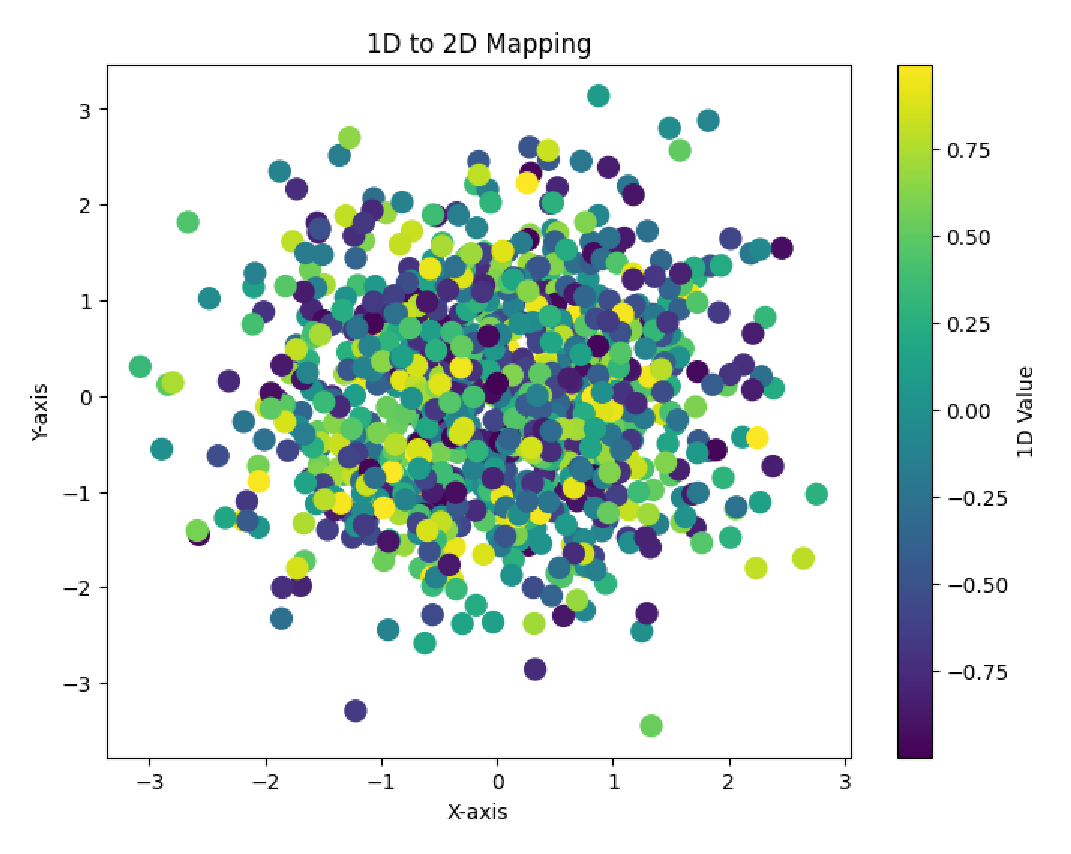
\includegraphics[width=3.0cm]{images/q5_1}}
  %  \vspace{1.5cm}
    \centerline{(a) mapping of output}\medskip
  \end{minipage}
  \hfill
  \begin{minipage}[c]{0.48\linewidth}
    \centering
    \centerline{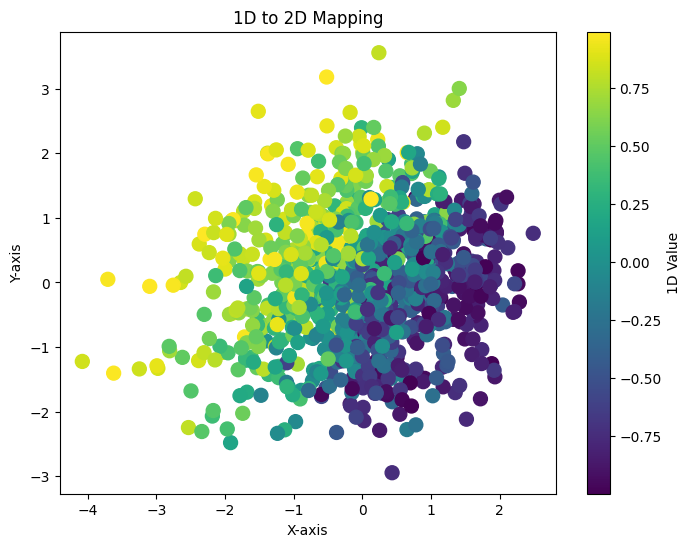
\includegraphics[width=3.0cm]{images/q5_2}}
  %  \vspace{1.5cm}
    \centerline{(b) mapping of prediction}\medskip
  \end{minipage}
  %
  \caption{Points mapped of Model 3}
  \label{fig:q5}
  %
  \end{figure}

\section{CONCLUSION}
\label{sec:conclusion}

To achieve {\bf not} the best rendering both in printed proceedings and electronic proceedings, we
strongly encourage you to use Times-Roman font.  In addition, this will give
the proceedings a more uniform look.  Use a font that is no smaller than nine
point type throughout the paper, including figure captions.

In nine point type font, capital letters are 2 mm high.  {\bf If you use the
smallest point size, there should be no more than 3.2 lines/cm (8 lines/inch)
vertically.}  This is a minimum spacing; 2.75 lines/cm (7 lines/inch) will make
the paper much more readable.  Larger type sizes require correspondingly larger
vertical spacing.  Please do not double-space your paper.  TrueType or
Postscript Type 1 fonts are preferred.

The first paragraph in each section should not be indented, but all the
following paragraphs within the section should be indented as these paragraphs
demonstrate.

\section{STATEMENT OF ALL TOOLS USED}
\label{sec:statementofalltoolsused}

Major headings, \cite{Lamp86} for example, "1. Introduction", should appear in all capital
letters, bold face if possible, centered in the column, with one blank line
before, and one blank line after. Use a period (".") after the heading number,
not a colon.

% To start a new column (but not a new page) and help balance the last-page
% column length use \vfill\pagebreak.
% -------------------------------------------------------------------------
%\vfill
%\pagebreak

\vfill\pagebreak

% References should be produced using the bibtex program from suitable
% BiBTeX files (here: strings, refs, manuals). The IEEEbib.bst bibliography
% style file from IEEE produces unsorted bibliography list.
% -------------------------------------------------------------------------
\bibliographystyle{IEEEbib}
\bibliography{strings,refs}

\end{document}
